
%opening
\title{Ranking der Vorschläge}
\author{Lothar Mödl, Burak Erol}

\chapter{Ranking der Vorschläge}

Die Suchergebnisse für einen Begriff oder  für Wortgruppen müssen nach den Interessen des Nutzers sortiert werden. Die Auswahl der Ergebnisse basiert auf verschiedenen Regeln. Diese Regeln sind Funktionen, die überprüfen, ob ein Kriterium erfüllt ist, oder nicht. Bei Vollendung einer Regel wird der Wert 1 oder 0 zurückgeliefert. 1 bedeutet, die Regel trifft zu und ist erfüllt, 0 bedeutet, die Regel wurde nicht erfüllt und trifft nicht zu. Für jeden Datensatz können alle Regeln durchlaufen werden, müssen aber nicht. Außerdem besitzt jede Regel eine Gewichtung, die aussagt, wie sehr diese Regel die Interessen des Nutzers wiederspiegelt. Nachdem alle Regeln abgeprüft wurden, wird der jeweilige Wert mit dem prozentualen Wert der Gewichtung multipliziert. Dies hat zur Folge, dass die negativ bewerteten Regeln eliminiert werden. Nach dieser Rechenoperation folgt eine Zweite. Diese legt fest, dass alle Teilergebnisse aufsummiert werden und im Anschluss durch die gesamte Anzahl aller abgeprüften Reglen dividiert wird. Der daraus resultierende Wert beschreibt als Prozentangabe, in wie fern dieser Datensatz den Nutzer interessieren könnte. Der oben genannte Prozess muss für jeden Datensatz wiederholt werden. Am Ende werden alle Ergebnisse sortiert, sodass das Ergebnis mit dem höchsten Prozentwert ganz oben landet und am Ende dem Nutzer präsentiert werden kann. 

\begin{figure}
	\centering
	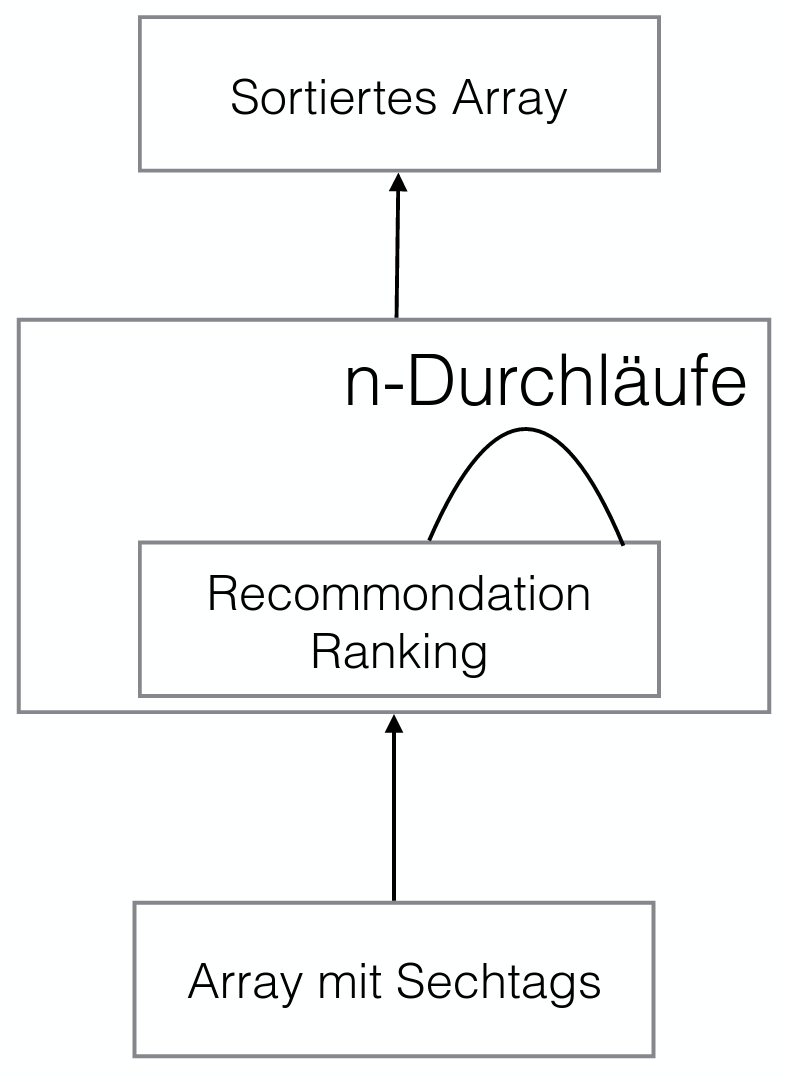
\includegraphics[width=10cm]{rankinguebersicht}
	\caption{Ablauf des Rankings}
	\label{fig:Rankingablauf}
\end{figure}

Dieses Diagramm stellt den allgemeinen Ablauf des Rankings dar. Im Folgenden wird das Recommendation Ranking im Detail erklärt. 

\begin{figure}
	\centering
	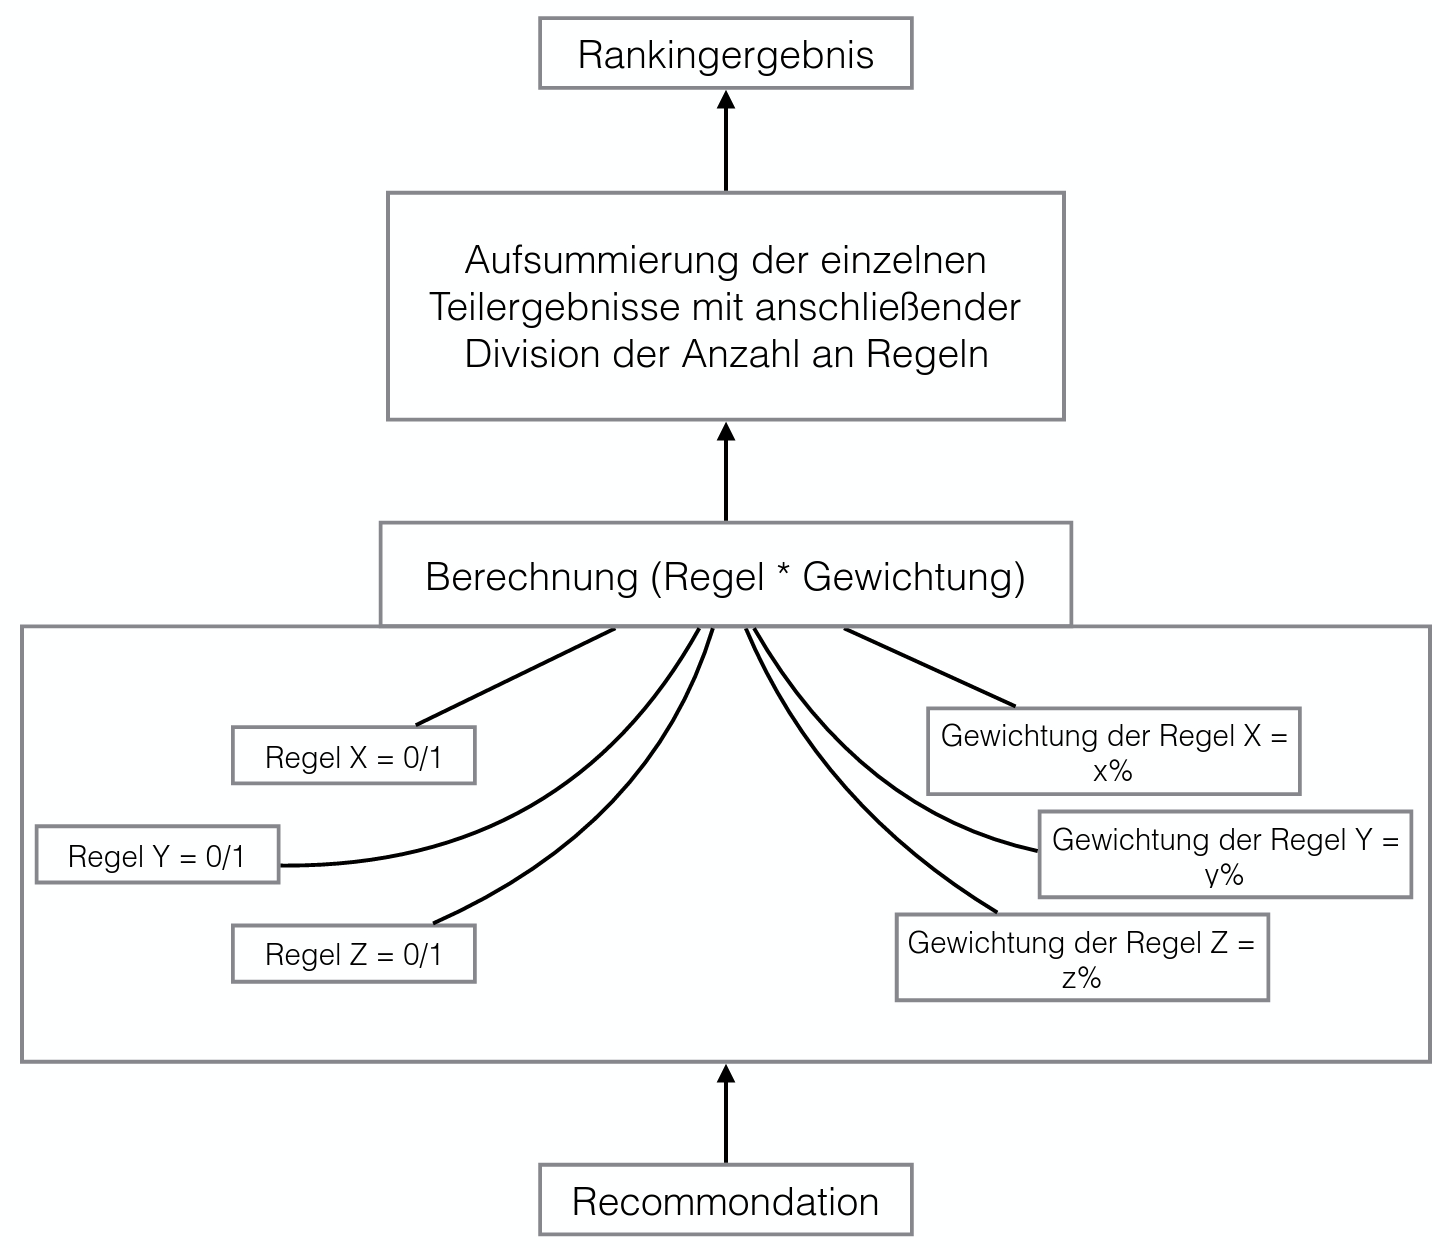
\includegraphics[width=15cm]{Ranking_Detail}
	\caption{Detailablauf Ranking}
	\label{fig:Detailablauf}
\end{figure}